

\section{분석}

\subsection{identification}

전파로 관측한 데이터는 시선방향에 대해 누적되고, 관찰자에 대한 상대 속도를 가진 물질의 분포를 알려준다. 원시성을 둘러싼 외피는 원시성에 대해 정적이거나 작은 속도로 수축하는 반면에 방출류는 원시성으로부터 두 극지방 방향으로 빠른 속도 성분을 가지고 멀어지므로 방출류의 축이 기울어져 있다면 관찰자를 향해 빠르게 접근하거나 멀어지는 것으로 보인다. 본 연구에서는 물질의 양이 적어 광학적 깊이가 깊기 때문에 외피를 추적하는 $^{13}CO$, $C^{18}O$ 데이터를 이용해서 line을 살펴보았다. 그리고 이를 Gaussian fitting 하여 원시성의 속도 center velocity($v_{cen}$)을 구하고 외피의 속도 분산을 나타내는 반치전폭(FWHM: Full Width Half Maximum)을 구했다. 외피가 아닌 red lobe의 $v_{out}$과 blue lobe의 $v_{in}$ 즉 적분 구간의 시작점은 $v_{cen}$로부터 FWHM만큼 떨어진 지점으로 지정하고, red lobe의 $v_{in}$과 blue lobe의 $v_{out}$은 각 lobe에 대한 오차($\sigma$)이하로 intensity가 떨어지는 지점을 직접 line으로 보면서 정하여 외피가 아닌 적색/청색편이된 성분의 속도 범위를 구하였다. 본 연구에서 관찰한 원시성들에 대한 속도 범위는 부록에 추가하였다.\\
방출류는 분자의 속도가 외피의 속도와 차이가 생겨 도플러 효과에 의해 시선방향으로 외피와는 다른 
주파수를 나타내기 때문에 $^{12}CO$ 방출선은 물질의 양이 많아 광학적 깊이가 얕아 방출류의 정보를 가진다. 또한 외피와의 속도 차이가 큰 영역에서 optically thin하기 때문에 앞에서 구한 식들의 가정에 맞다. 따라서 $^{12}CO$ 데이터의 값을 앞에서 정한 구간에서 적분한 값을 사용하여 적색/청색편이된 성분을 관찰할 수 있는 contour map을 그렸다. 여기서 원시성을 중심으로 서로 반대 방향으로 방출류가 존재하는지 확인하였다. 여기서 보이는 red, blue lobe들이 관찰하고자 하는 원시성으로부터 나오는 방출류인지 확인하기 위해 ccontour map에서 나타나는 red, blue peak와 관찰하고자 하는 원시성의 위치 center에 대해 line을 그렸다. $^{12}CO$와 $^{13}CO$, $C^{18}O$ 천이 선으로 red peak, blue peak, center의 line profile을 그려 관찰하는 원시성으로부터 나온 방출류가 맞는지 확인하였다. 그렇게 확인된 방출류에 대해 기둥 밀도와 방출류의 세기를 구해 분석하였다.\\
여기서 속도 성분 (v + Δv)사이에 있는 물질의 양은 $(\ref{column density})$와 같고, $T_{MB}$는 관측온도$T_A$를 main beam efficiency로 나눠줬을 때의 온도이다. 그리고 방출류의 세기는 $(\ref{FCO})$으로 힘의 단위 [$M_{\odot} km s^{-1} yr^{-1}$]로 계산된다.\cite{Hatchell2}
\\
SED는 http://vizier.u-strasbg.fr/vizier/sed/ 에서 얻은 데이터를 이용하여 그렸다. 관측하고자 하는 원시성으로부터 5 arcsec 위치에서 관측한 다양한 데이터들을 이용하여 SED를 그리고, 그 중 2$\mu m $에서 20$\mu m$ 사이에 있는 데이터들에 대해 선형 추세선을 그려 $\alpha$값을 구했다. 그리고 $\alpha$값을 이용하여 각 대상의 진화단계를 분류하고 알려져있는 classification과 비교해 보았다. 


\section{결과}

\begin{table}[h!]
	\begin{center}
		\begin{tabular}{c|c|c|c|c}
			\toprule
			& \multicolumn{2}{c|}{\textbf{coordinates}} & $\mathbf{L_{bol}}$ & $\mathbf{T_{bol}}$\\
			\textbf{Name} & \textbf{RA} & \textbf{Dec} & ${[L_{\odot}]}$ & $[K]$\\
			\midrule
			\multicolumn{5}{c}{Orion A Cloud}\\
			\midrule
			\centering
			FIR2 & 05:35:24.3 & -5:08:33.3 & 5.68 & 100.6\\
			FIR3 & 05:35:27.5 & -5:09:32.5 & 360.86 & 71.5\\
			FIR6b & 05:35:23.4 & -5:12:03.2 & 21.93 & 54.1\\
			MMS2 & 05:35:18.3 & -05:00:34.8 & 20.11 & 186.3\\
			MMS5 & 05:35:22.4 & -05:01:14.1 & 15.81 & 42.4\\
			MMS9 & 05:35:26.0 & -05:05:42.4 & 8.91 & 38.1\\
			\midrule
			\multicolumn{5}{c}{$\rho$ Ophiuchus Cloud}\\
			\midrule
			\centering
			Elias 32 & 16:27:28.6 & -24:27:19.8 & 1.5 & 620\\
			IRS 46 & 16:27:29.7 & -24:39:16.0 & 0.19 & 280\\
			VLA 1623 & 16:26:26.4 & -24:24:30.9 & 1.0 & 35\\
			BBRCG 24 & 16:27:09.0 & -24:34:08.0 & 0.8 & 1600\\
		\end{tabular}
	\end{center}
	\caption{관측된 원시성들의 정보. 위는 Orion A Cloud에서 관측된 6개의 원시성, 아래는 $\rho$ Ophiuchus Cloud에서 관측된 4개의 원시성이다.}
\end{table}



\begin{figure}[h!]
	\begin{center}
		\begin{tabular}{ccc}
			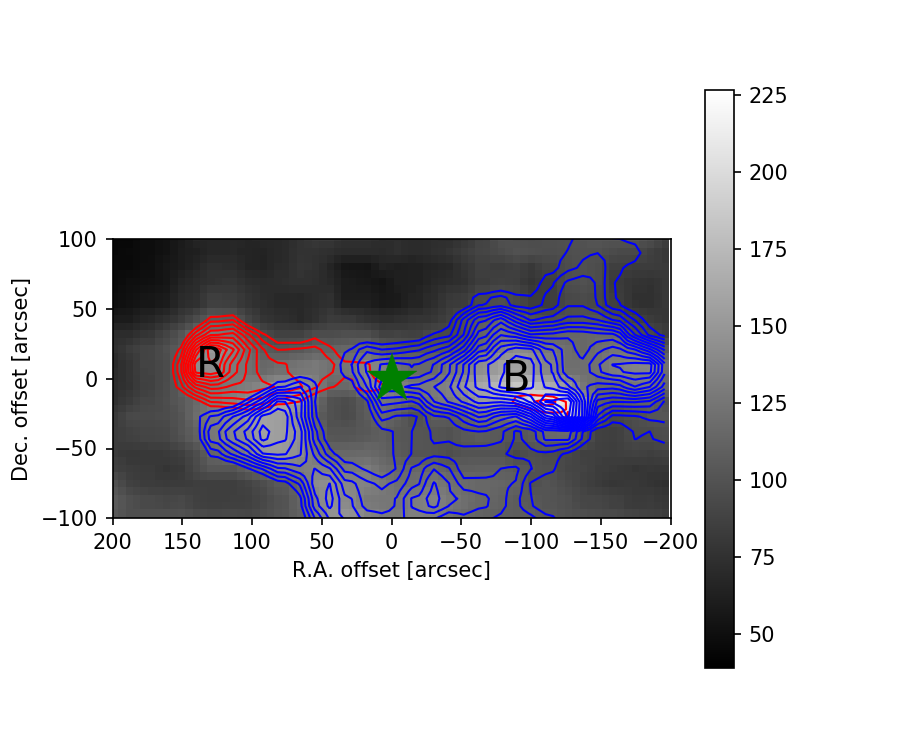
\includegraphics[height=6.5cm]{Orion_12CO_intmap.png} & 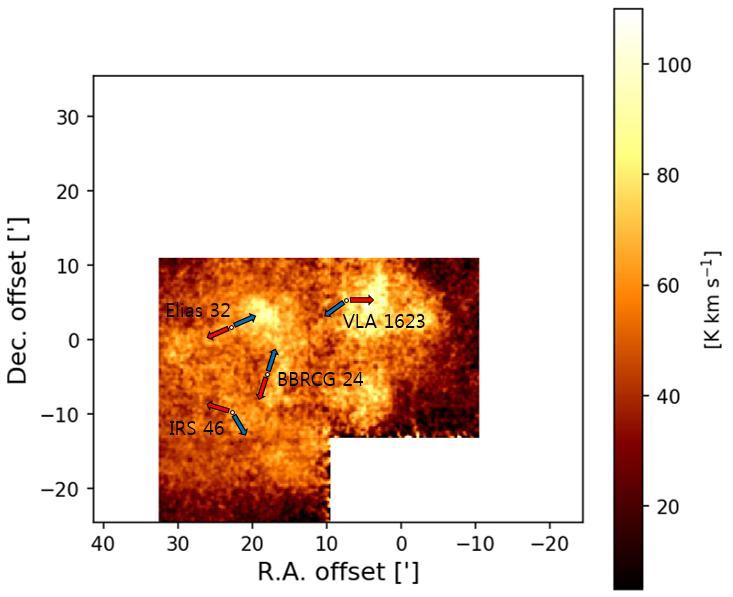
\includegraphics[height=6.5cm]{Oph_12CO_intmap.png}
		\end{tabular}
	\end{center}
	\caption{Orion A Cloud $^{12}CO$ intergrated intensity map(좌) $\rho$ Ophiuchus Cloud $^{12}CO$ intergrated intensity map(우). 좌측의 그림은 Orion A Cloud에서 관측한 북쪽 영역의 원시성들의 위치와 이름을 표시하였다. 우측의 그림은 $\rho$ Ophiuchus Cloud의 L1688 영역에서 관측한 원시성들의 위치와 이름, 방출류의 방향을 표시하였다.}
\end{figure}

본 연구에서는 Orion A Cloud의 북쪽 영역에 대해 Takahashi에서 ASTE를 이용한 $^{12}CO$ J=3-2 관측 데이터를 사용하여 발견한 10개의 원시성에 대해 IRAM $^{12}CO$ J=2-1 관측 데이터를 사용해서 6개의 원시성만 방출류를 검출할 수 있었다.\cite{Takahashi}
그리고 $\rho$ Ophiuchus Cloud의 L1688 영역에 대해서는 Marel에서 JCMT를 이용한 $^{12}CO$ J=3-2 관측 데이터를 사용하여 발견한 13개의 원시성에 대해 $^{12}CO$ J=1-0 관측 데이터를 사용한 본 연구에서는 오직 4개의 원시성만 방출류를 검출 할 수 있었다. \cite{Marel}
\\
이후에 나오는 Countour map에서 Orion A Cloud의 경우 10'가 실제 길이로는 1.25pc, $\rho$ Ophiuchus Cloud에서는 10'가 실제 길이로는 0.40pc이다. 그리고 Line profile에서 검은선은 $^{12}CO$ 천이 선, 초록선은 $^{13}CO$ 천이 선, 갈색선은 $C^{18}O$ 천이 선의 line이며 파랑색과 빨강색 점선은 blue, red lobe의 속도 범위를 나타낸 것이다.


\subsection{Orion A Cloud}

\begin{figure}[h!]
	\begin{center}
		\begin{tabular}{ccc}
			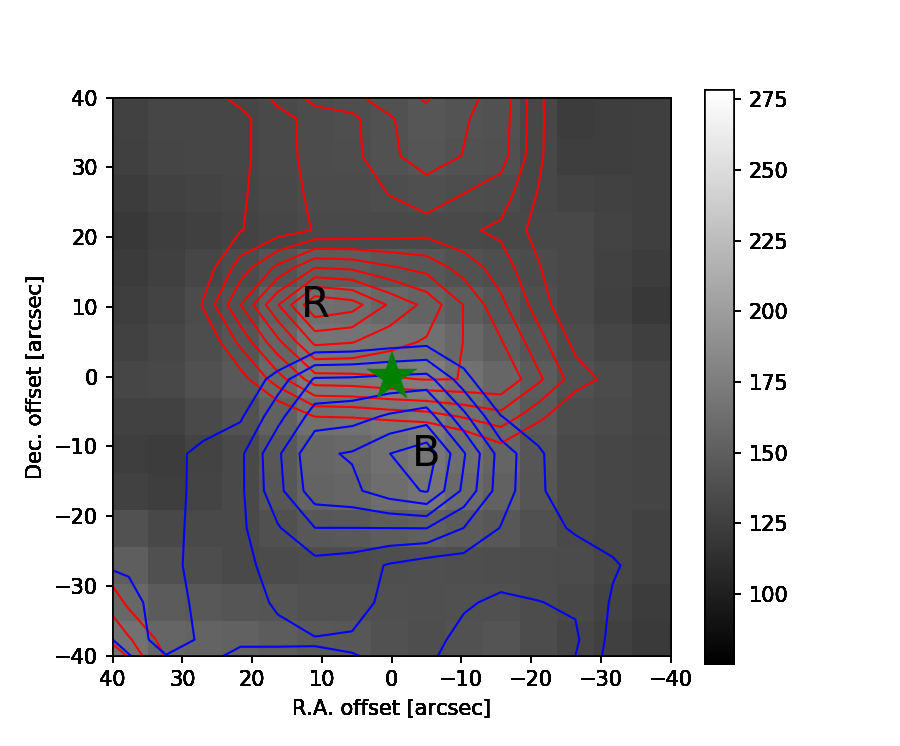
\includegraphics[width=5cm]{Orion_12CO2-1_FIR2_rbcontour_400_modified.png} &   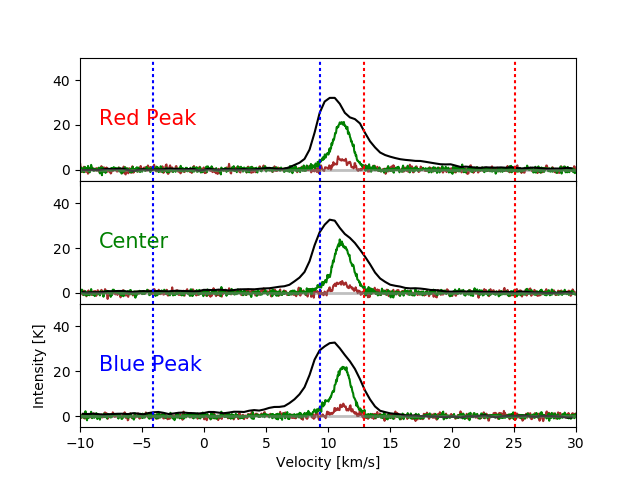
\includegraphics[width=5cm]{Orion_12CO2-1_FIR2_line_profile_400.png} &
			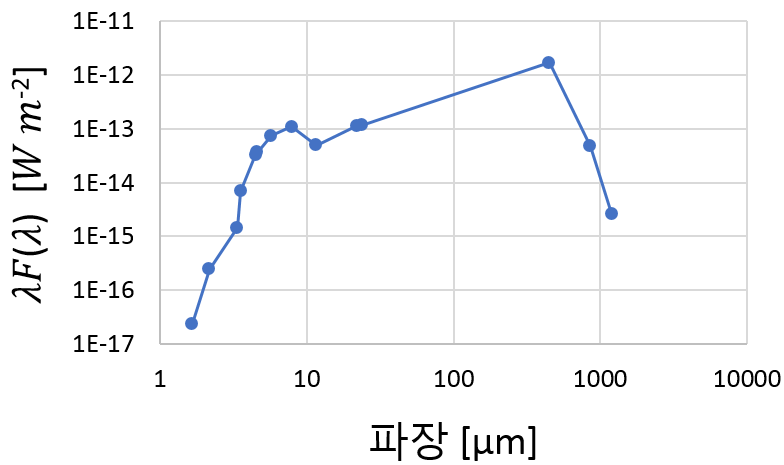
\includegraphics[width=5cm]{FIR2_SED.PNG} \\
		\end{tabular}
		\caption{FIR2의 contour map(왼쪽)과 line profile(중간), SED(오른쪽)이다. Red lobe는 contour level이 오차의 60배부터 140배까지 9단계, blue lobe는 100배부터 160배까지 7단계로 나누어서 그림을 그렸다.}
	\end{center}
\end{figure}

\begin{figure}[h!]
	\begin{center}
		\begin{tabular}{ccc}
			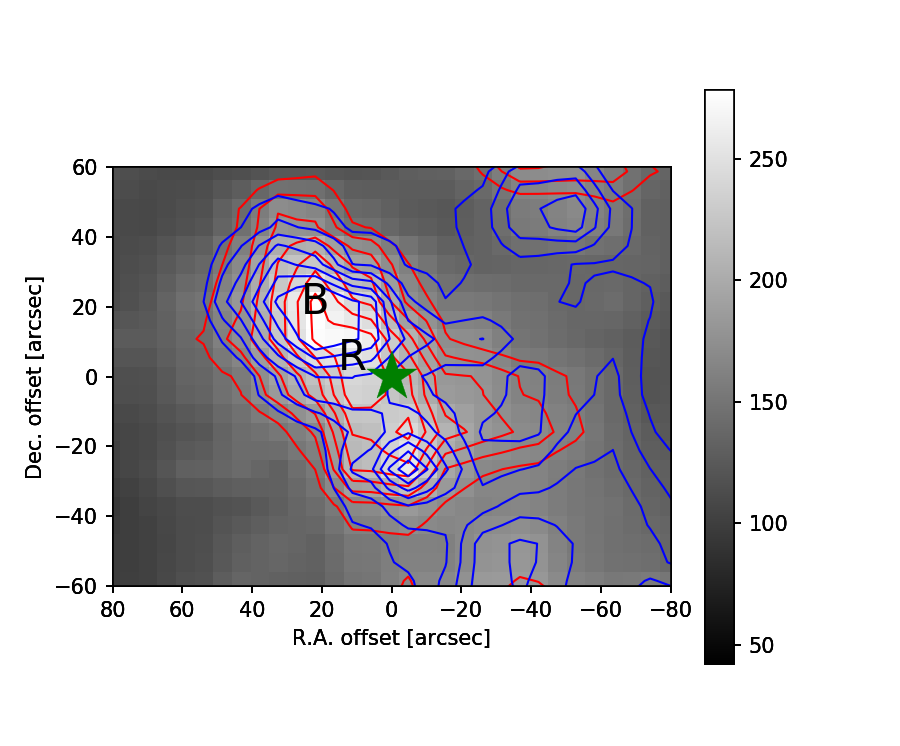
\includegraphics[width=5cm]{Orion_12CO2-1_FIR3_rbcontour_400_modified.png} &   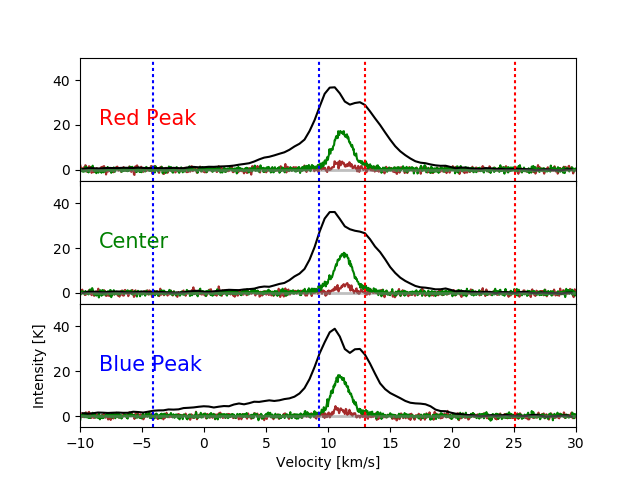
\includegraphics[width=5cm]{Orion_12CO2-1_FIR3_line_profile_400.png} &
			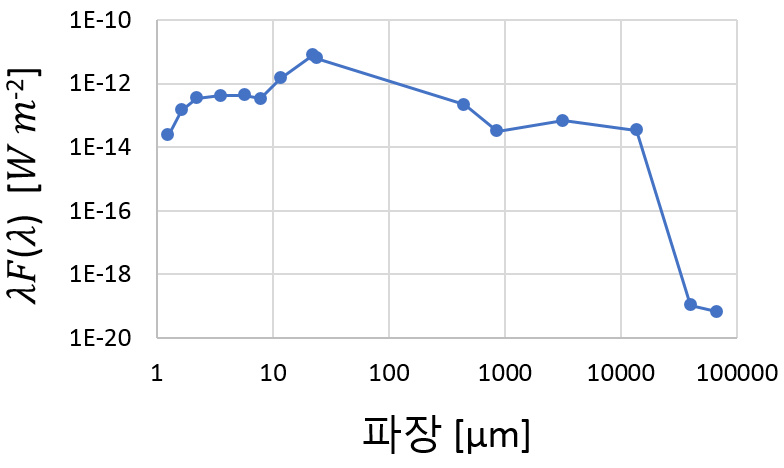
\includegraphics[width=5cm]{FIR3_SED.PNG} \\
		\end{tabular}
		\caption{FIR3의 contour map(왼쪽)과 line profile(중간), SED(오른쪽)이다. Red lobe는 contour level이 오차의 40배부터 160배까지 7단계, blue lobe는 60배부터 180배까지 7단계로 나누어서 그림을 그렸다.}
	\end{center}
\end{figure}

\begin{figure}[h!]
	\begin{center}
		\begin{tabular}{ccc}
			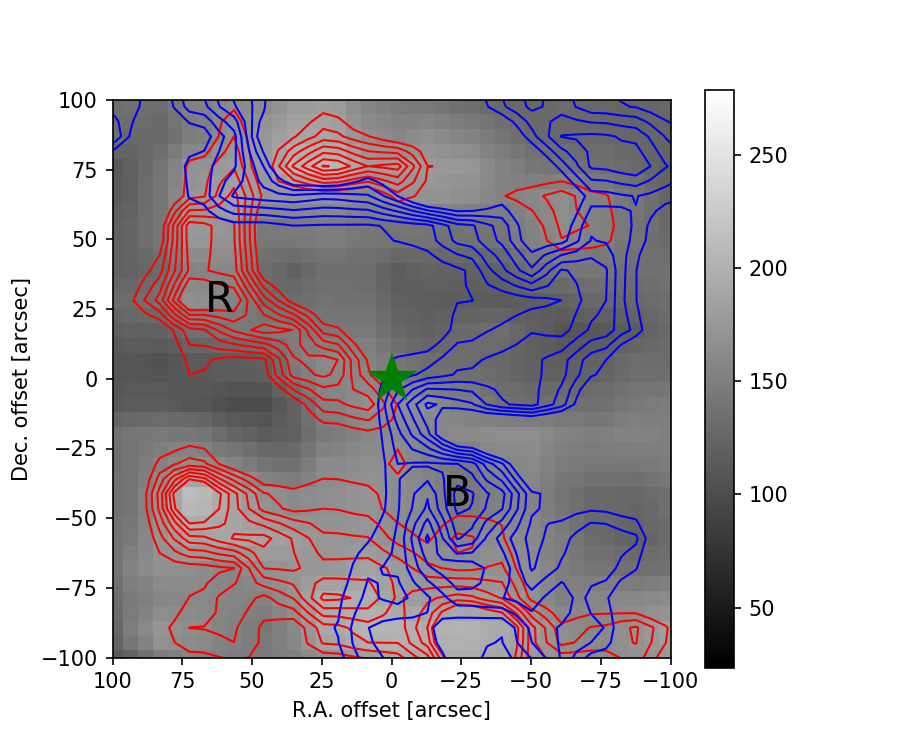
\includegraphics[width=5cm]{Orion_12CO2-1_FIR6b_rbcontour_400_modified.png} &   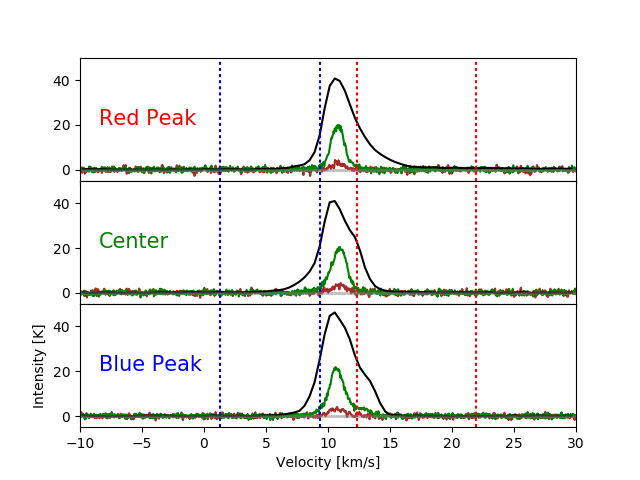
\includegraphics[width=5cm]{Orion_12CO2-1_FIR6b_line_profile_400.png} &
			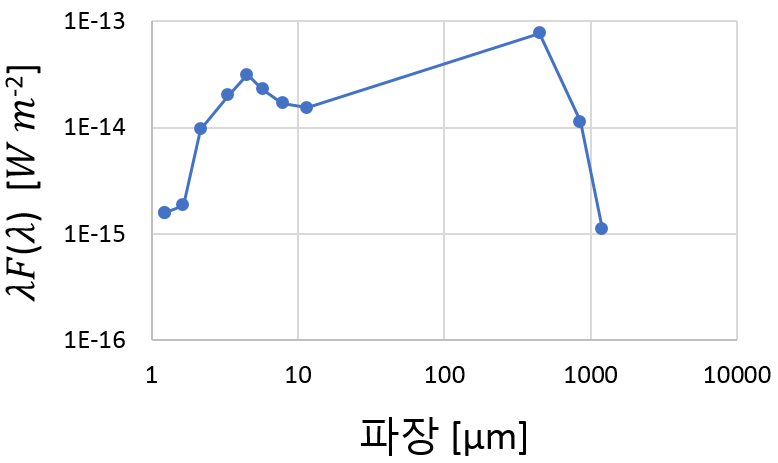
\includegraphics[width=5cm]{FIR6b_SED.PNG}\\
		\end{tabular}
		\caption{FIR6b의 contour map(왼쪽)과 line profile(중간), SED(오른쪽)이다. Red lobe는 contour level이 오차의 45배부터 105배까지 7단계, blue lobe는 50배부터 110배까지 7단계로 나누어서 그림을 그렸다.}
	\end{center}
\end{figure}

\begin{figure}[h!]
	\begin{center}
		\begin{tabular}{ccc}
			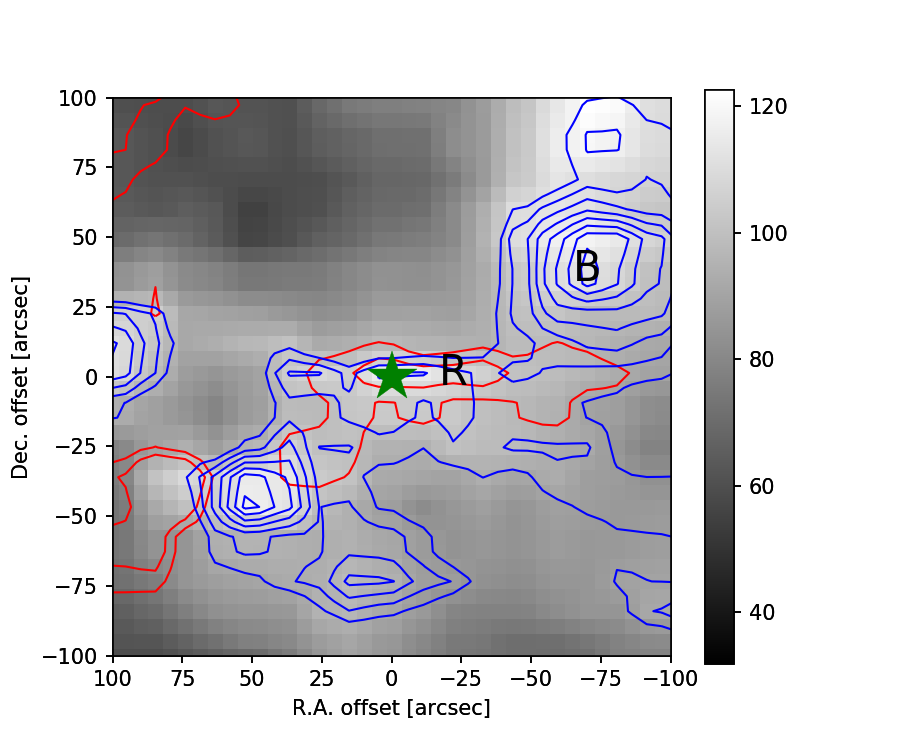
\includegraphics[width=5cm]{Orion_12CO2-1_MMS2_rbcontour_400_modified.png} &   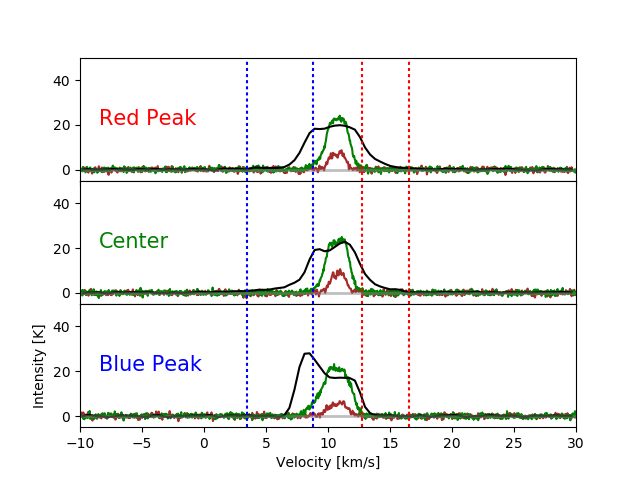
\includegraphics[width=5cm]{Orion_12CO2-1_MMS2_line_profile_400.png} &
			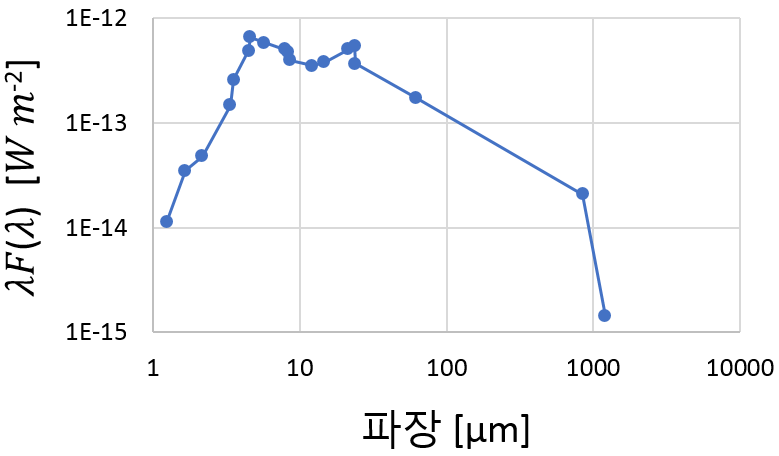
\includegraphics[width=5cm]{MMS2_SED.PNG}\\
		\end{tabular}
		\caption{MMS2의 contour map(왼쪽)과 line profile(중간), SED(오른쪽)이다. Red lobe는 contour level이 오차의 30배부터 40배까지 2단계, blue lobe는 60배부터 130배까지 8단계로 나누어서 그림을 그렸다.}
	\end{center}
\end{figure}

\begin{figure}[h!]
	\begin{center}
		\begin{tabular}{ccc}
			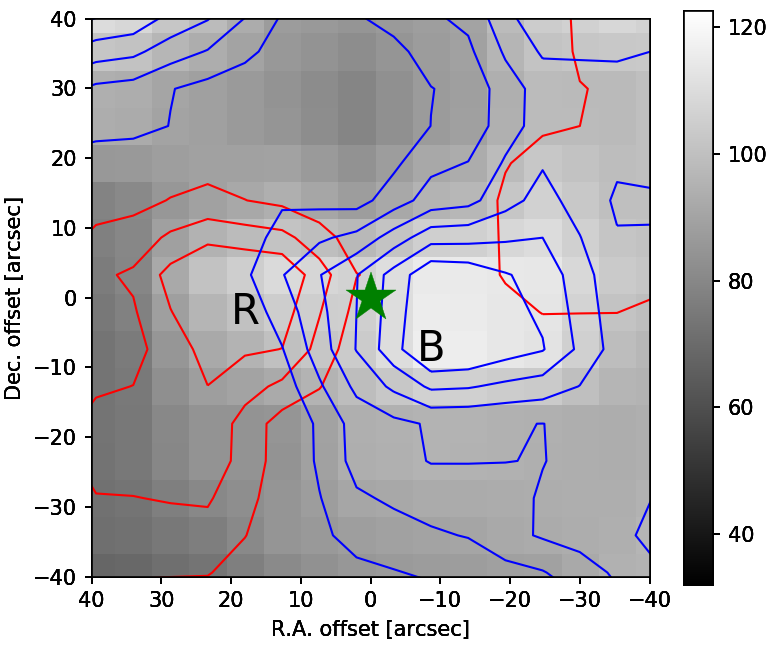
\includegraphics[width=5cm]{Orion_12CO2-1_MMS5_rbcontour_400_modified.png} &   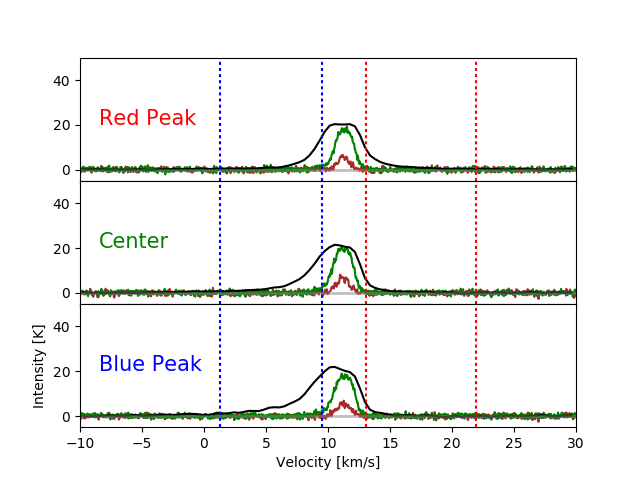
\includegraphics[width=5cm]{Orion_12CO2-1_MMS5_line_profile_400.png} &
			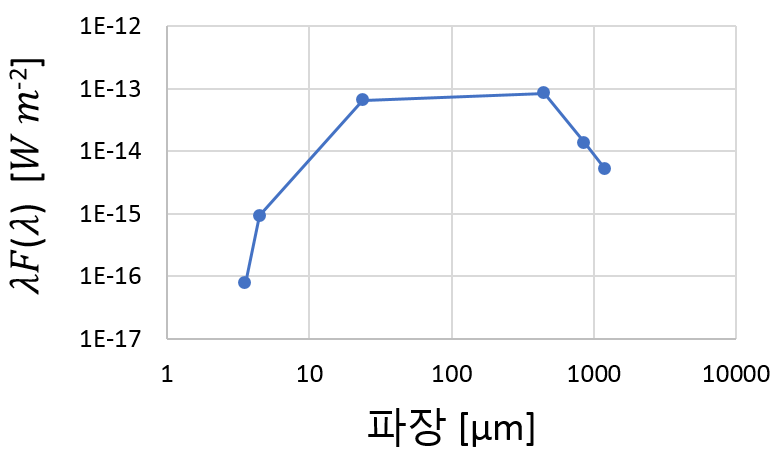
\includegraphics[width=5cm]{MMS5_SED.PNG}\\
		\end{tabular}
		\caption{MMS5의 contour map(왼쪽)과 line profile(중간), SED(오른쪽)이다. Red lobe는 contour level이 오차의 20배부터 30배까지 2단계, blue lobe는 40배부터 90배까지 6단계로 나누어서 그림을 그렸다.}
	\end{center}
\end{figure}

\begin{figure}[h!]
	\begin{center}
		\begin{tabular}{ccc}
			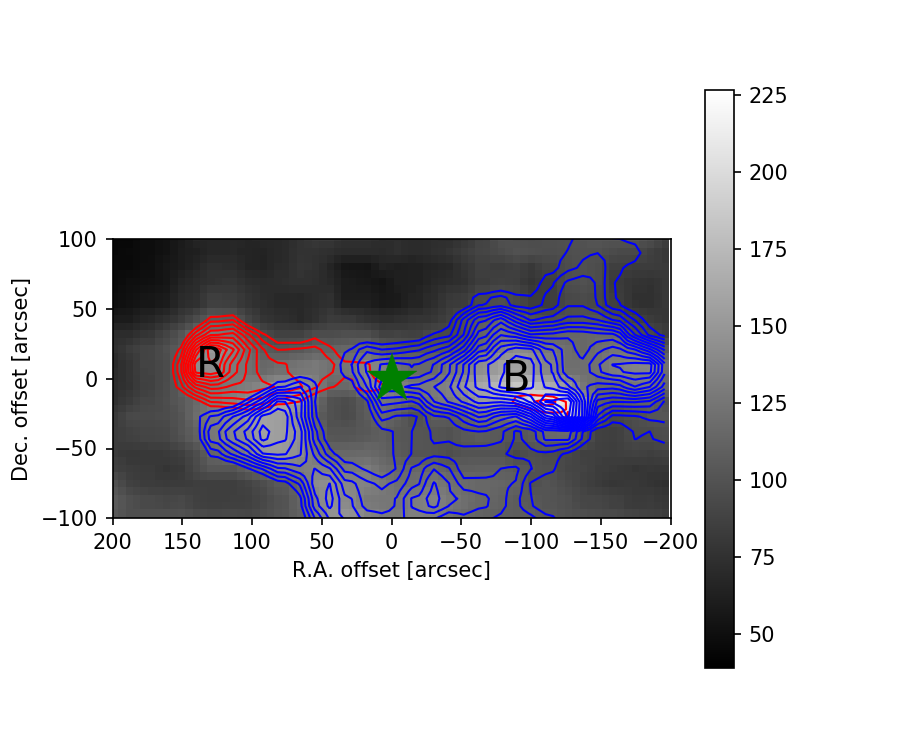
\includegraphics[width=5cm]{Orion_12CO2-1_MMS9_rbcontour_400_modified.png} &   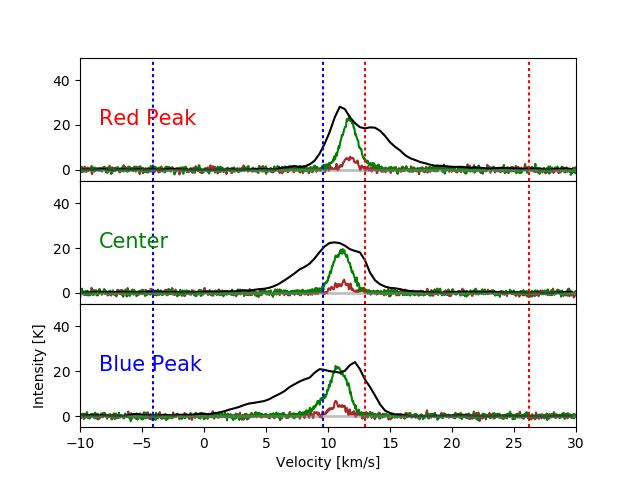
\includegraphics[width=5cm]{Orion_12CO2-1_MMS9_line_profile_400.png} &
			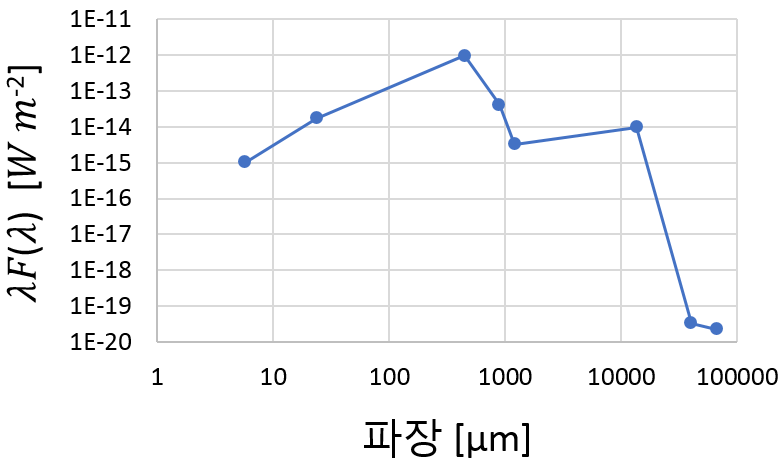
\includegraphics[width=5cm]{MMS9_SED.PNG}\\
		\end{tabular}
		\caption{MMS9의 contour map(왼쪽)과 line profile(중간), SED(오른쪽)이다. Red lobe는 contour level이 오차의 50배부터 140배까지 10단계, blue lobe는 60배부터 200배까지 15단계로 나누어서 그림을 그렸다.}
	\end{center}
\end{figure}

\clearpage
\newpage   
FIR2의 contour map을 살펴보면 N-S 방향으로 강한 방출류가 보인다. 방출류의 크기가 약 30 arcsec정도로 다른 방출류들보다 훨씬 작다. 본 연구의 결과가 Takahashi보다 약 3배 더 약하게 나타났다. Aso는 이 천체에 대하여 분석을 하지 않았다. SED의 기울기 $\alpha$는 3.12으로 Class I으로 분류하였다. Furlan에서도 Class I으로 분류하였다.\cite{HerschelFurlan} 

FIR3의 contour map을 살펴보면  red lobe와 blue lobe의 중심이 거의 같은 위치에 있다. 방출류가 거의 시선방향과 나란하다는 것을 알 수 있다. 본 연구의 결과가 Takahashi보다 약 20배 더 약하게 나타났다. Takahashi는 red와 blue lobe를 각각 2개씩 관측했다. Aso는 이 천체에 대하여 분석을 하지 않았다.  SED의 기울기 $\alpha$는 1.51으로 Class I으로 분류하였다. Furlan에서도 Class I으로 분류하였다.\cite{HerschelFurlan} 

FIR6b의 contour map을 살펴보면 주변의 다른 별들로 인해서 방출류 구조 말고 다른 별들에서 나온 방출류로 인한 선들이 많이 보인다. NW-SE 방향으로 방출류가 관측이 된다. 본 연구의 결과가 Takahashi보다 약 4배 더 약하게 나타났다. Aso는 이 천체에 대하여 분석을 하지 않았다. SED의 기울기 $\alpha$는 1.20으로 Class I으로 분류하였다. Furlan에서는 Class 0으로 분류하였다.\cite{HerschelFurlan} 

MMS2의 contour map을 살펴보면 red lobe와 blue lobe가 둘 다 별을 기준으로 동쪽에 있는 특이한 모양을 하고 있다. SW 방향에 보이는 방출류 구조는 MMS5로 인한 방출류이다. 아마 이것에 의해 방출류가 영향을 받아 치우쳐졌을 가능성이 있다. 본 연구의 결과가 Takahashi보다 약 4배 더 약하게 나타났다. J=1-0 을 사용한 Aso보다 약 1.8배 더 강하게 나타났다. Aso는 MMS2, MMS3, MMS4 세 개의 원시성을 하나의 원시성으로 간주하고 방출류를 계산했다.\cite{Aso} SED의 기울기 $\alpha$는 1.23으로 Class I으로 분류하였다. Furlan에서는 Flat으로 분류하였다.\cite{HerschelFurlan} 

MMS5의 contour map을 살펴보면 E-W 방향으로 방출류가 관측이 된다. blue lobe가 red lobe보다 더 강하게 관측된다. 본 연구의 결과가 Takahashi보다 약 4배 더 약하게 나타났다. Aso보다 약 10\% 강하게 나타났다.\cite{Aso} SED의 기울기 $\alpha$가 3.17로 Class I로 분류되어야 하지만 $2.2\mu m$와 $20 \mu m$ 사이의 관측 데이터의 값이 $10^{-15}$ Wm$^{-2}$정도로 매우 작게 나타났기 때문에 Class 0으로 분류하였다. Furlan에서는 Class I으로 분류하였다.\cite{HerschelFurlan} 

MMS9의 contour map을 살펴보면  E-W 방향으로 강한 방출류가 나오는 것을 볼 수 있다. Takahashi(2008)에서는 red lobe를 두개 관측했는데, 본 연구의 관측 자료에서도 blue lobe의 중심 부근에서 작은 red lobe가 존재하는것을 알 수 있다. 그 세기는 main red lobe보다 10배 정도 더 작은것으로 관측되었다. 본 연구의 결과가 Takahashi보다 약 20배 더 약하게 나타났다. Takahashi는 2개의 red lobe를 관측했다.  Aso의 결과에 비해서는 약 6.7배 약하게 나타났다.\cite{Aso} SED의 기울기 $\alpha$는 1.53으로 Class I으로 분류하였다. Furlan에서는 Class 0으로 분류하였다.\cite{HerschelFurlan} 
\\

각 원시성들의 line profile에 나타난 $^{13}CO$와 $C^{18}O$ 천이 선을 보면 red peak, center, blue peak 세 지점에서 모두 비슷한 개형이 나타났다. 따라서 각 원시성 주변의 red, blue lobe가 본 연구에서 관찰한 원시성으로부터 나온 방출류라는 것을 알 수 있다. 그리고 SED로부터 분류한 진화단계가 일부 원시성들은 Furlan의 결과와 다르게 나타났는데, Furlan은 각 원시성들을 bolometric temperature을 기준으로 분류했기 때문에 본 연구에서 SED를 이용해서 구한 classification과 차이가 있을 수 있다.

\clearpage
\newpage   


\subsection{방출류의 세기}
\begin{table}[h]
	\begin{center}
		\begin{tabular}{c|c|c|c}
			\toprule
			\textbf{Name} &$\mathbf{F_{R}}$ & $\mathbf{F_{B}}$ & $\mathbf{F_{CO}}$\\
			& \multicolumn{3}{c}{[M$_{\odot}$ km s$^{-1}$ yr$^{-1}$]}\\
			\midrule
			\multicolumn{4}{c}{Orion A Cloud}\\
			\midrule
			FIR2 & 1.14E-05 & 3.28E-05 & 4.42E-05\\
			FIR3 & 4.77E-03 & 7.43E-03 & 1.22E-04\\
			FIR6b & 1.13E-05 & 1.18E-05 & 2.31E-05\\
			MMS2 & 1.14E-05 & 4.50E-05 & 5.64E-05\\
			MMS5 & 5.80E-06 & 1.55E-05 & 2.13E-05\\
			MMS9 & 3.67E-06 & 1.09E-05 & 1.46E-05\\
			\midrule
			\multicolumn{4}{c}{$\rho$ Ophiuchus Cloud}\\
			\midrule
			Elias 32 & 1.77E-06 & 1.01E-05 & 1.19E-05\\
			IRS 46 & 4.56E-07 & 7.14E-07 & 1.17E-06\\
			VLA 1623 & 2.42E-06 & 3.15E-06 & 5.57E-06\\
			BBRCG 24 & 3.78E-07 & 8.19E-07 & 1.20E-06\\
		\end{tabular}
	\end{center}
	\caption{관측된 원시성들의 방출류의 세기}
\end{table}

표에서 $F_R$와 $F_B$는 각각 red, blue lobe의 방출류의 세기를 구한것이다.(\ref{FCO}) $F_{CO}$는 두 값을 더한 값으로 원시성이 방출해내는 총 방출류의 세기이다. 두 영역의 방출류를 비교해 보면 $\rho$ Ophiuchus Cloud은 Orion A Cloud보다 질량이 작고 광도가 낮은 별들이 탄생하는 영역으로 방출류의 세기 또한 작게 나타났다.\\

\section{토의}

\subsection{기존 연구와 비교}

\begin{figure}[h]
	\begin{center}
		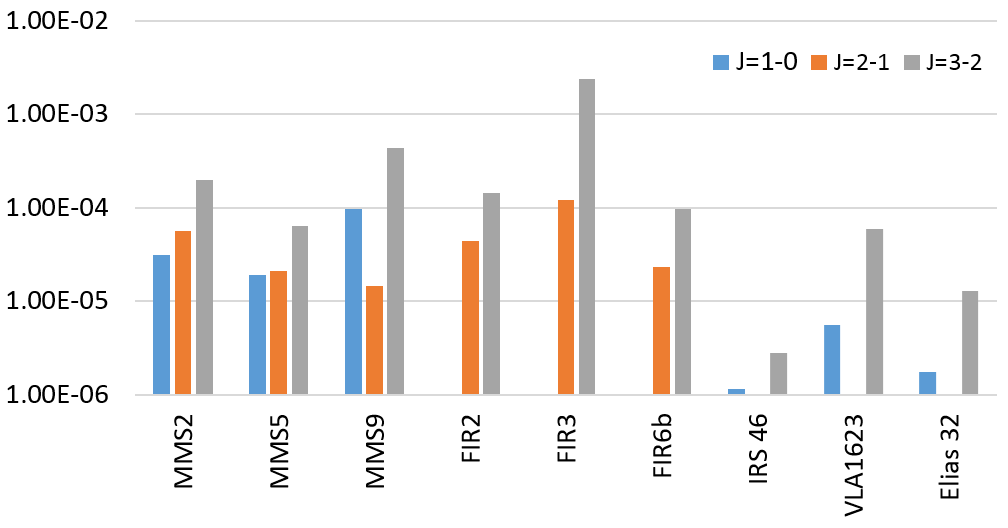
\includegraphics[height=7cm]{COFCO.PNG}
	\end{center}
	\caption{Orion A Cloud와 $\rho$ Ophiuchus Cloud에서 관측한 원시성들에 대해 $^{12}CO$ J=3-2와 J=2-1, J=1-0 방출선으로 구해진 방출류의 세기. Orion A Cloud의 경우 J=2-1, $\rho$ Ophiucus Cloud의 경우 J=1-0이 본 연구에서 구한 방출류의 세기이다.}
\end{figure}

Orion A Cloud를 $^{12}CO$ J=1-0, J=3-2 관측 데이터로 구한 방출류의 세기는 각각 Aso, Takahashi의 결과를 참고하였고, $\rho$ Ophiuchus Cloud를 $^{12}CO$ J=3-2 관측 데이터로 구한 방출류의 세기는 Marel, Nakamura의 결과를 참고하였다.\cite{Aso}\cite{Takahashi}\cite{Marel}\cite{Nakamura} 두 영역에서 모두 MMS9을 제외한 원시성에서는 높은 천이 선일수록 방출류의 세기가 크게 나타났다.
\\
또한 Orion A Cloud 북쪽 영역에 대해 Takahashi에서 $^{12}CO$ J=3-2 관측 데이터를 사용하여 알려진 10개의 원시성 중 본 연구에서 사용한 $^{12}CO$ J=2-1 관측 데이터로는 6개의 방출류만 찾을 수 있었다. 그리고 $\rho$ Ophiuchus Cloud L1688에 대해서도 Marel에서 $^{12}CO$ J=3-2 관측 데이터를 사용하여 발견한 13개의 원시성에 비해 본 연구에서는 $^{12}CO$ J=1-0 관측 데이터를 사용한 결과 오직 4개의 원시성만 관측 가능하였다.\cite{Takahashi}\cite{Marel} 그리고 Orion A Cloud의 경우 본 연구에서 사용한 데이터의 beam size는 11 arcsec로 22 arcsec였던 Takahashi의 데이터보다 더 정밀하기 때문에 온도가 높은 더 안쪽 영역을 추적한 것으로 볼 수 있다. 따라서 높은 $CO$ 천이 선일수록 상대적으로 보다 따뜻한 가스를 추적하고, 방출류를 더 잘 추적한다고 알려져 있는데, Orion A Cloud와 $\rho$ Ophiuchus Cloud 영역에서 이를 확인 할 수 있었다. 하지만 $^{12}CO$ J=2-1, J=1-0 천이 선 또한 $^{12}CO$ J=3-2 천이 선과 비슷한 정도로 충분히 방출류를 추적할 수 있음을 알 수 있다.


\subsection{두 영역의 광도에 따른 방출류의 세기}

\begin{figure}[h]
	\centering
	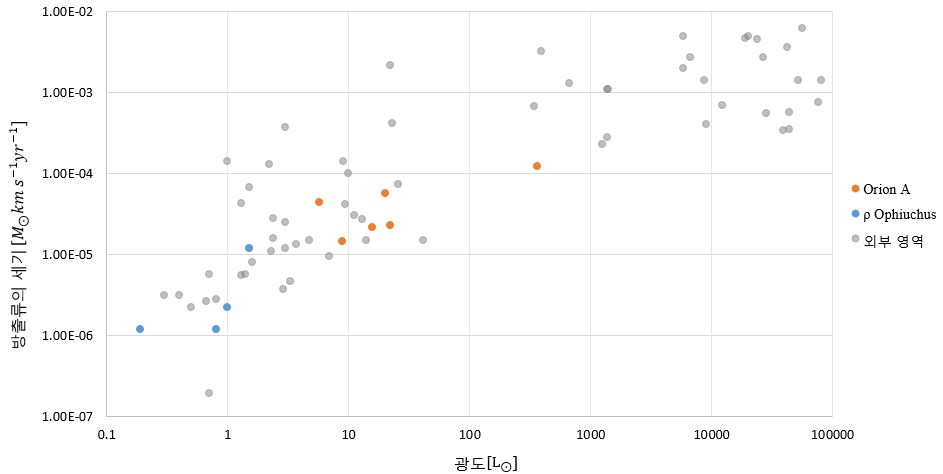
\includegraphics[height=8cm]{luminosity-outflowforce.JPG}
	\caption{광도-방출류의 세기 관계 그래프}
\end{figure}

이 그래프는 Takahashi, Bontemps, Hogerheijde, Zhang 논문 에서 발견된 다양한 별 탄생 영역 안의 원시성들의 방출류의 세기와 본 연구에서 구한 Orion A Cloud와 $\rho$ Ophiuchus Cloud 영역 안의 원시성들의 방출류의 세기를 가지고 광도와의 관계를 나타낸 것이다.\cite{Takahashi} \cite{Bontemps} \cite{Hogerheijde} \cite{Zhang} 원시성의 광도는 Spitzer와 Herschel 망원경으로 관측된 값들을 사용하였다.\cite{OphDunham} \cite{Spitzer} \cite{HerschelFurlan} Orion A Cloud는 중간 정도 질량의 별들이 형성되는 지역이고 보다 큰 광도와 방출류의 세기를 보인다. $\rho$ Ophiuchus Cloud는 낮은 질량의 별들이 형성되는 지역이고, Orion A Cloud 영역보다는 상대적으로 낮은 광도와 방출류의 세기를 보인다. 관찰한 두 지역의 원시성들에 대해 모두 방출류의 세기와 원시성의 광도가 비례한다는 사실을 재확인 할 수 있었다.